% this is a simplified version of 
% https://github.com/yihui/knitr/blob/master/inst/examples/knitr-beamer.Rnw
\documentclass{beamer}\usepackage[]{graphicx}\usepackage[]{color}
%% maxwidth is the original width if it is less than linewidth
%% otherwise use linewidth (to make sure the graphics do not exceed the margin)
\makeatletter
\def\maxwidth{ %
  \ifdim\Gin@nat@width>\linewidth
    \linewidth
  \else
    \Gin@nat@width
  \fi
}
\makeatother

\definecolor{fgcolor}{rgb}{0.345, 0.345, 0.345}
\newcommand{\hlnum}[1]{\textcolor[rgb]{0.686,0.059,0.569}{#1}}%
\newcommand{\hlstr}[1]{\textcolor[rgb]{0.192,0.494,0.8}{#1}}%
\newcommand{\hlcom}[1]{\textcolor[rgb]{0.678,0.584,0.686}{\textit{#1}}}%
\newcommand{\hlopt}[1]{\textcolor[rgb]{0,0,0}{#1}}%
\newcommand{\hlstd}[1]{\textcolor[rgb]{0.345,0.345,0.345}{#1}}%
\newcommand{\hlkwa}[1]{\textcolor[rgb]{0.161,0.373,0.58}{\textbf{#1}}}%
\newcommand{\hlkwb}[1]{\textcolor[rgb]{0.69,0.353,0.396}{#1}}%
\newcommand{\hlkwc}[1]{\textcolor[rgb]{0.333,0.667,0.333}{#1}}%
\newcommand{\hlkwd}[1]{\textcolor[rgb]{0.737,0.353,0.396}{\textbf{#1}}}%
\let\hlipl\hlkwb

\usepackage{framed}
\makeatletter
\newenvironment{kframe}{%
 \def\at@end@of@kframe{}%
 \ifinner\ifhmode%
  \def\at@end@of@kframe{\end{minipage}}%
  \begin{minipage}{\columnwidth}%
 \fi\fi%
 \def\FrameCommand##1{\hskip\@totalleftmargin \hskip-\fboxsep
 \colorbox{shadecolor}{##1}\hskip-\fboxsep
     % There is no \\@totalrightmargin, so:
     \hskip-\linewidth \hskip-\@totalleftmargin \hskip\columnwidth}%
 \MakeFramed {\advance\hsize-\width
   \@totalleftmargin\z@ \linewidth\hsize
   \@setminipage}}%
 {\par\unskip\endMakeFramed%
 \at@end@of@kframe}
\makeatother

\definecolor{shadecolor}{rgb}{.97, .97, .97}
\definecolor{messagecolor}{rgb}{0, 0, 0}
\definecolor{warningcolor}{rgb}{1, 0, 1}
\definecolor{errorcolor}{rgb}{1, 0, 0}
\newenvironment{knitrout}{}{} % an empty environment to be redefined in TeX

\usepackage{alltt}
\IfFileExists{upquote.sty}{\usepackage{upquote}}{}
\begin{document}

\title{Introducci\'on a la Gen\'omica \\ UNAL nov 2017}
\author{Alejandro Caceres \\ ISGlobal, Barcelona}


\maketitle

% very important to use option [fragile] for frames containing code output!

\begin{frame}[fragile]
\frametitle{datos de SNPs}
Cada programa tiene un formato diferente y es importante saber cambiar de formato
\begin{itemize}
\item {\tt PLINK}: Es un programa compilado, corre por la linea de comandos y es muy rapido. Es particularmente util para manejar las bases de datos en si, exlcuir sujetos, seleccionar SNPs. No tiene la versatilidad de R para explorar graficos, crear nuevas funciones o hacer graficos, pero es muy utilizado y con experiencia en computacion facil de hacer pipelines.

\item {\tt snpStats} (bioconductor): Tiene varias funciones para ver la estructura de los datos (linakage-disequilibium, pca, Fst), y hace analisis de asociacion en base de datos grandes, pero no prueba diferentes modelo de herencia. Usa un fromato especial (raw data).

\item {\tt snpAssoc} (r-cran): versatil para probar diferentes modelos de herencia, pero las funciones no estan optimizadas para menejar matrices muy grandes. 

\item {\tt tabix} : un programa para gestionar datos en formato VCF usado por los 1000 genomas  
 
\end{itemize}
\end{frame}

\begin{frame}[fragile]
\frametitle{PLINK}
Es un programa por linea de comandos desarrollado por Chrostopher Chang.

\begin{figure}[htbp]
\begin{center}
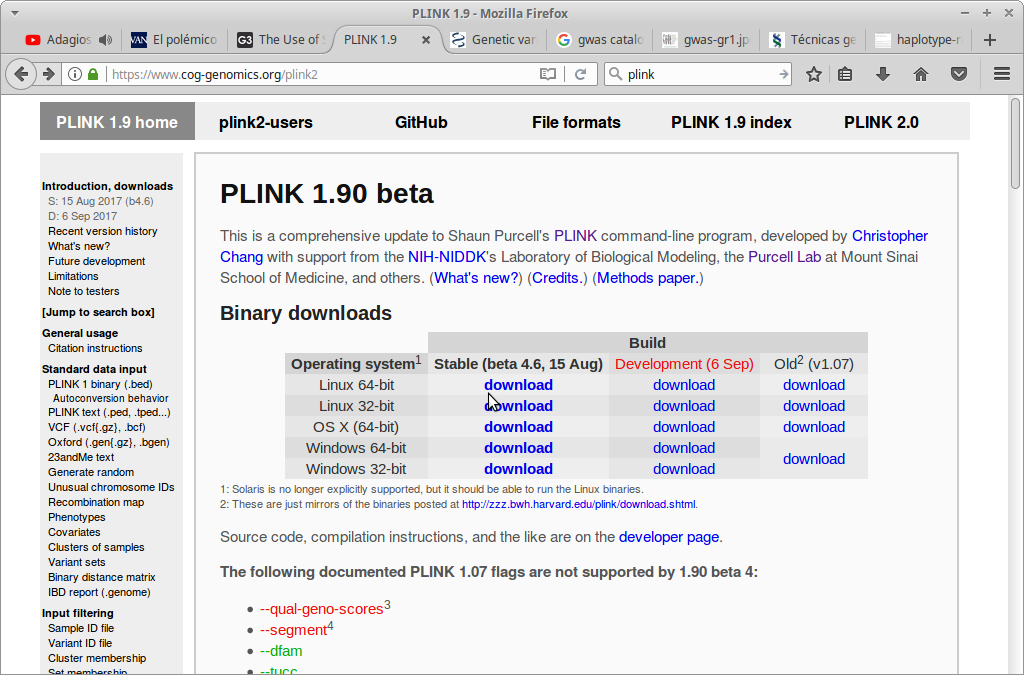
\includegraphics[width=.8\linewidth]{plink.png}
\end{center}
\end{figure}

Tiene una documentaci\'on muy completa
\end{frame}


\begin{frame}[fragile]
\frametitle{PLINK}
PLINK tiene dos formatos
\begin{itemize}
\item {\tt .bed, .bim, .fam}: es el mas usado y separa la informaci\'on en tres archivos genotipos (.bed), anotacion de SNPs (.bim), fenotipos (.fam)  

\item {\tt .ped, .map}: .ped son los .fam en las primeras columnas y .map es una versi\'on con menos info que .bim
 
\end{itemize}
\end{frame}

\begin{frame}[fragile]
\frametitle{PLINK}

Para cambiar los cambiar el formatos de misDatos.ped y misDatos.map a misDatos.bed, misDatos.bim y misDatos.fam

\begin{verbatim}
plink --file misDatos --make-bed --out misDatos
\end{verbatim}

\begin{figure}[htbp]
\begin{center}
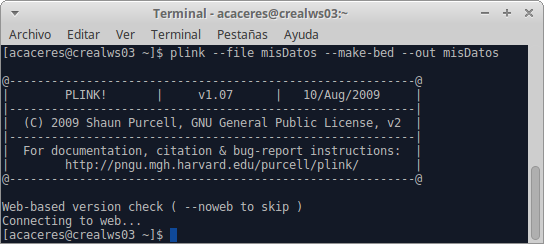
\includegraphics[width=.8\linewidth]{command.png}
\end{center}
\end{figure}

\end{frame}



\begin{frame}[fragile]
\frametitle{Datos de SNPs}

Despues del preprocesamiento de los datos, los datos que se obtienen es de un gentipo por individuo. Si tenemos 1 millon de SNPs y 1000 individuos, esto es tipicamente una matriz de $10^3 \times 10^6$. Hay diferentes formas de organizar estos datos
 
\begin{verbatim}
        rs33  rs36  rs43
NA090   A/C   G/G   T/A ...
NA091   A/A   G/G   T/A ...
NA092   A/A   G/C   T/A ...
NA093   A/C   C/C   A/A ...
...
\end{verbatim}
\end{frame}



\begin{frame}[fragile]
\frametitle{Datos de SNPs}

Hay diferentes formas de organizar estos datos
 
\begin{verbatim}
        rs33  rs36  rs43
NA090   A/C   G/G   T/A ...
NA091   A/A   G/G   T/A ...
NA092   A/A   G/C   T/A ...
NA093   A/C   C/C   A/A ...
...
\end{verbatim}
Una forma eficiante es llamar 0:homocigoto, 1:heterocigoto y 2:heterocigoto variante.

\begin{itemize}
\item para SNP=rs33 el alelo mas frecuente es A y el menos frecuente es C. \newline Entonces:  A/A=0, A/C=1, CC=2
\item para SNP=rs36 el alelo mas frecuente es G y el menos frecuente es C. \newline Entonces:  G/G=0, G/C=1, CC=2

\end{itemize}
\end{frame}



\begin{frame}[fragile]
\frametitle{Datos tipicos de SNPs (PLINK) formato bed}
\begin{itemize}
\item Datos de los genotipos (datos.bed)
\begin{verbatim}
        rs33 rs36 rs43
NA090   1    0    1 ...
NA091   0    0    1 ...
NA092   0    1    1 ...
NA093   1    2    2 ...
...
\end{verbatim}
\end{itemize}
\end{frame}

\begin{frame}[fragile]
\frametitle{Datos tipicos de SNPs (PLINK) formato bed}
\begin{itemize}
\item Datos con la anotacion de SNPs (datos.bim)
\begin{verbatim}
chr snp   mor   pos   allele1 allele2
1   rs33  0     1034  A       C
1   rs36  0     2000  G       C
1   rs43  0     10056 T       A 
...
\end{verbatim}
\end{itemize}
\end{frame}

\begin{frame}[fragile]
\frametitle{Datos tipicos de SNPs (PLINK) formato bed}
\begin{itemize}
\item Datos con los fenotipos (datos.fam)
\begin{verbatim}
ID  FAMID sex asthma  BMI-z
NA090 1   1    1      1.2
NA091 1   1    0      1.5
NA092 2   0    0      0.9
NA093 2   0    1      1
\end{verbatim}

\end{itemize}
\end{frame}

\begin{frame}[fragile]
\frametitle{PLINK}
en https://www.cog-genomics.org/plink/1.9/resources hay datos de prueba para aprender a usar PLINK

Si PLINK esta instalado
\begin{itemize}
\item bajar  1kg$\_$phase1$\_$chr22.tar.gz
\item descomprimir
\item ejecutar 
\end{itemize}

{\tt plink --bfile 1kg$\_$phase1$\_$chr22 --make-bed --chr 22 --out mydata --to-mb 20}

Esto selecciona unos datos del cromosoma 22 hasta 20 Mb y los guarda en mydata.bed, mydata.fam y mydata.bim
\end{frame}


\begin{frame}[fragile]
\frametitle{SNPstats}
Es un programa en R (bioconductor)

\begin{figure}[htbp]
\begin{center}
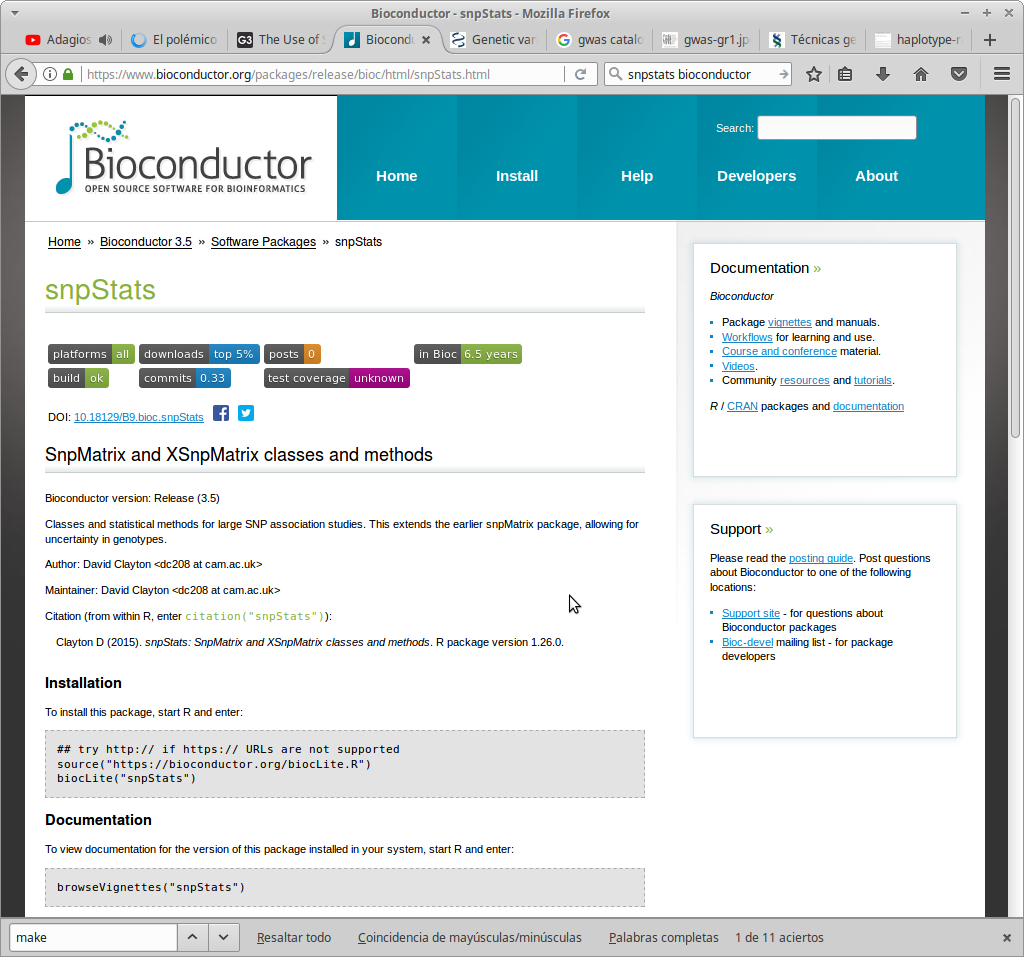
\includegraphics[width=.6\linewidth]{snpstats.png}
\end{center}
\end{figure}

tiene la ventaja de que esta en ambiente R y se pueden usar otros paquetes de bioconductor
\end{frame}



\begin{frame}[fragile]
\frametitle{SNPstats}

se instalala como desde R por medio de los comandos

\begin{knitrout}\footnotesize
\definecolor{shadecolor}{rgb}{0.969, 0.969, 0.969}\color{fgcolor}\begin{kframe}
\begin{alltt}
\hlkwd{source}\hlstd{(}\hlstr{"https://bioconductor.org/biocLite.R"}\hlstd{)}
\hlkwd{biocLite}\hlstd{(}\hlstr{"snpStats"}\hlstd{)}
\end{alltt}
\end{kframe}
\end{knitrout}
\end{frame}


\begin{frame}[fragile]
\frametitle{SNPstats}

la librer\'ia se carga con
\begin{knitrout}\footnotesize
\definecolor{shadecolor}{rgb}{0.969, 0.969, 0.969}\color{fgcolor}\begin{kframe}
\begin{alltt}
\hlkwd{library}\hlstd{(}\hlstr{"snpStats"}\hlstd{)}
\end{alltt}


{\ttfamily\noindent\itshape\color{messagecolor}{\#\# Loading required package: survival}}

{\ttfamily\noindent\itshape\color{messagecolor}{\#\# Loading required package: Matrix}}\end{kframe}
\end{knitrout}

cargemos los datos
\begin{knitrout}\footnotesize
\definecolor{shadecolor}{rgb}{0.969, 0.969, 0.969}\color{fgcolor}\begin{kframe}
\begin{alltt}
\hlstd{snp}\hlkwb{<-}\hlkwd{read.plink}\hlstd{(}\hlstr{"datos/mydata"}\hlstd{)}
\end{alltt}


{\ttfamily\noindent\color{warningcolor}{\#\# Warning: non-unique value when setting 'row.names': '.'}}

{\ttfamily\noindent\bfseries\color{errorcolor}{\#\# Error in `row.names<-.data.frame`(`*tmp*`, value = value): duplicate 'row.names' are not allowed}}\end{kframe}
\end{knitrout}
Un error t\'ipico de cuando algunos SNPs no est\'an anotados
\end{frame}


\begin{frame}[fragile]
\frametitle{SNPstats}
Veamos cuales son los SNPs que estan anotados

\begin{knitrout}\footnotesize
\definecolor{shadecolor}{rgb}{0.969, 0.969, 0.969}\color{fgcolor}\begin{kframe}
\begin{alltt}
\hlstd{bim}\hlkwb{<-}\hlkwd{read.table}\hlstd{(}\hlstr{"datos/mydata.bim"}\hlstd{,}\hlkwc{as.is}\hlstd{=}\hlnum{TRUE}\hlstd{)}

\hlstd{rs}\hlkwb{<-}\hlstd{bim[,}\hlnum{2}\hlstd{]}
\hlstd{tb}\hlkwb{<-}\hlkwd{table}\hlstd{(rs)}
\hlstd{dup}\hlkwb{<-}\hlstd{tb[tb}\hlopt{>}\hlnum{1}\hlstd{]}
\hlstd{selrs}\hlkwb{<-}\hlstd{rs[}\hlopt{!}\hlstd{rs}\hlopt\hlkwd{names}\hlstd{(dup)]}

\hlkwd{head}\hlstd{(rs)}
\end{alltt}
\begin{verbatim}
## [1] "rs149201999" "rs146752890" "rs139377059" "rs188945759" "rs6518357"  
## [6] "rs62224609"
\end{verbatim}
\end{kframe}
\end{knitrout}

\end{frame}

\begin{frame}[fragile]
\frametitle{SNPstats}
Lamos los SNPs anotados con la apoci\'on {\tt select.snps}
\begin{knitrout}\footnotesize
\definecolor{shadecolor}{rgb}{0.969, 0.969, 0.969}\color{fgcolor}\begin{kframe}
\begin{alltt}
\hlstd{snp}\hlkwb{<-}\hlkwd{read.plink}\hlstd{(}\hlstr{"datos/mydata"}\hlstd{,} \hlkwc{select.snps} \hlstd{= selrs)}
\hlkwd{names}\hlstd{(snp)}
\end{alltt}
\begin{verbatim}
## [1] "genotypes" "fam"       "map"
\end{verbatim}
\end{kframe}
\end{knitrout}
\end{frame}

\begin{frame}[fragile]
\frametitle{SNPstats}
\begin{knitrout}\footnotesize
\definecolor{shadecolor}{rgb}{0.969, 0.969, 0.969}\color{fgcolor}\begin{kframe}
\begin{alltt}
\hlstd{snp}\hlopt{$}\hlstd{genotypes}
\end{alltt}
\begin{verbatim}
## A SnpMatrix with  1092 rows and  43067 columns
## Row names:  HG00096 ... NA20828 
## Col names:  rs149201999 ... rs145875228
\end{verbatim}
\end{kframe}
\end{knitrout}
\begin{knitrout}\footnotesize
\definecolor{shadecolor}{rgb}{0.969, 0.969, 0.969}\color{fgcolor}\begin{kframe}
\begin{alltt}
\hlkwd{head}\hlstd{(snp}\hlopt{$}\hlstd{fam)}
\end{alltt}
\begin{verbatim}
##         pedigree  member father mother sex affected
## HG00096       NA HG00096   <NA>   <NA>   1       NA
## HG00097       NA HG00097   <NA>   <NA>   2       NA
## HG00099       NA HG00099   <NA>   <NA>   2       NA
## HG00100       NA HG00100   <NA>   <NA>   2       NA
## HG00101       NA HG00101   <NA>   <NA>   1       NA
## HG00102       NA HG00102   <NA>   <NA>   2       NA
\end{verbatim}
\end{kframe}
\end{knitrout}

\begin{knitrout}\footnotesize
\definecolor{shadecolor}{rgb}{0.969, 0.969, 0.969}\color{fgcolor}\begin{kframe}
\begin{alltt}
\hlkwd{head}\hlstd{(snp}\hlopt{$}\hlstd{map)}
\end{alltt}
\begin{verbatim}
##             chromosome    snp.name cM position allele.1 allele.2
## rs149201999         22 rs149201999 NA 16050408        C        T
## rs146752890         22 rs146752890 NA 16050612        G        C
## rs139377059         22 rs139377059 NA 16050678        T        C
## rs188945759         22 rs188945759 NA 16050984        G        C
## rs6518357           22   rs6518357 NA 16051107        A        C
## rs62224609          22  rs62224609 NA 16051249        C        T
\end{verbatim}
\end{kframe}
\end{knitrout}
\end{frame}


\begin{frame}[fragile]
\frametitle{SNPstats}
se pueden guardar como binarios de R snp.RData
\begin{knitrout}\footnotesize
\definecolor{shadecolor}{rgb}{0.969, 0.969, 0.969}\color{fgcolor}\begin{kframe}
\begin{alltt}
\hlkwd{save}\hlstd{(snp,} \hlkwc{file}\hlstd{=}\hlstr{"datos/mydata.RData"}\hlstd{)}
\end{alltt}
\end{kframe}
\end{knitrout}

tambi\'en se pueden guardar datos de snpStats en PLINK con {\tt write.plink}
\end{frame}


\begin{frame}[fragile]
\frametitle{SNPstats}

Estos son solo genotipos guardados en binario {\tt snp.RData} 
\begin{knitrout}\footnotesize
\definecolor{shadecolor}{rgb}{0.969, 0.969, 0.969}\color{fgcolor}\begin{kframe}
\begin{alltt}
\hlkwd{load}\hlstd{(}\hlstr{"datos/snp.RData"}\hlstd{)}
\end{alltt}
\end{kframe}
\end{knitrout}

\begin{knitrout}\footnotesize
\definecolor{shadecolor}{rgb}{0.969, 0.969, 0.969}\color{fgcolor}\begin{kframe}
\begin{alltt}
\hlstd{snp}
\end{alltt}
\begin{verbatim}
## A SnpMatrix with  1500 rows and  439 columns
## Row names:  1 ... 1500 
## Col names:  1 ... 439
\end{verbatim}
\end{kframe}
\end{knitrout}

\end{frame}



\begin{frame}[fragile]
\frametitle{1000 Genomes}
Repositorio de datos de los 1000 genomas donde se pueden descargar los datos de 2504 individuos

\begin{figure}[htbp]
\begin{center}
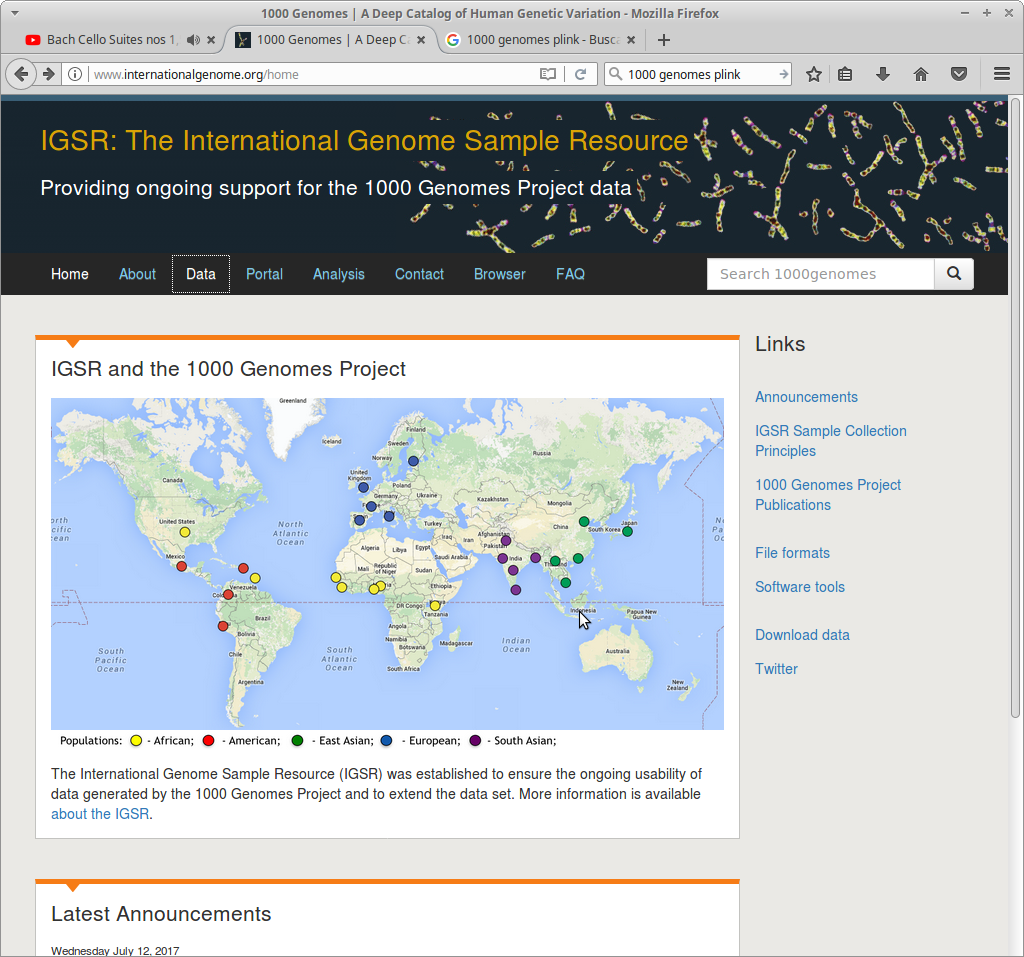
\includegraphics[width=.6\linewidth]{home1k.png}
\end{center}
\end{figure}
Hay un servidor ftp para descargar datos 
Los archivos son enormes, pero se puden leer por regiones con Tabix
\end{frame}



\begin{frame}[fragile]
\frametitle{1000 Genomes}
Tambi\'en hay un browser para bajar datos de regiones \begin{figure}[htbp]
\begin{center}
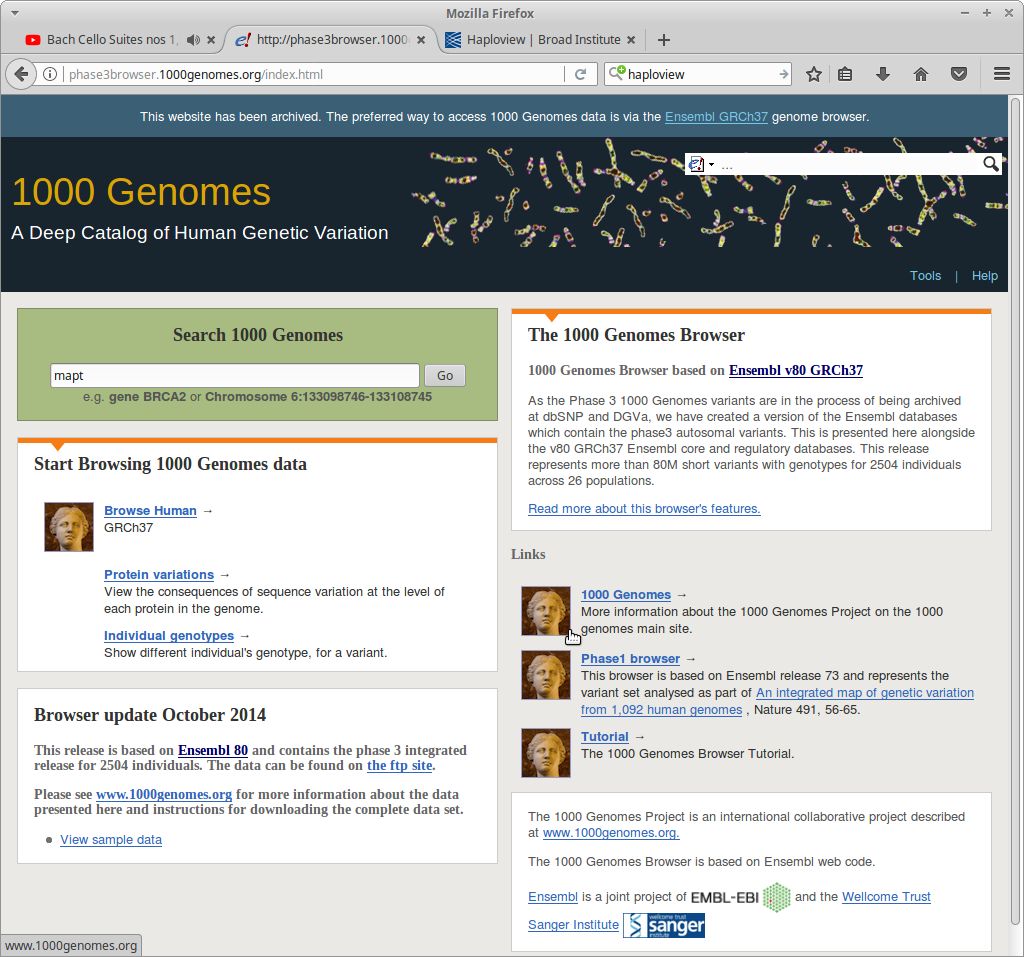
\includegraphics[width=.7\linewidth]{mapt.png}
\end{center}
\end{figure}

\end{frame}



\begin{frame}[fragile]
\frametitle{1000 Genomes}
obtengamos datos para \emph{MAPT}
\begin{figure}[htbp]
\begin{center}
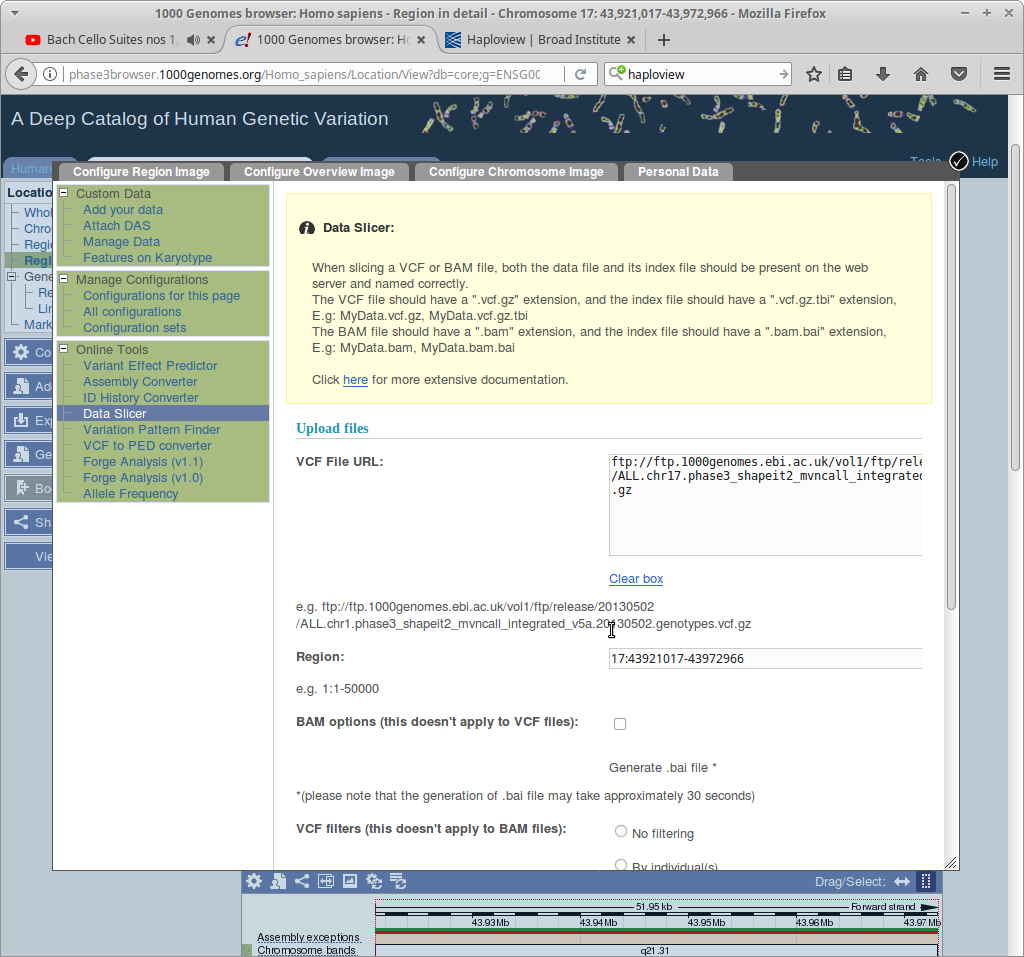
\includegraphics[width=.7\linewidth]{getvcf.png}
\end{center}
\end{figure}
\end{frame}


\begin{frame}[fragile]
\frametitle{1000 Genomes}
Formato VCF
\begin{figure}[htbp]
\begin{center}
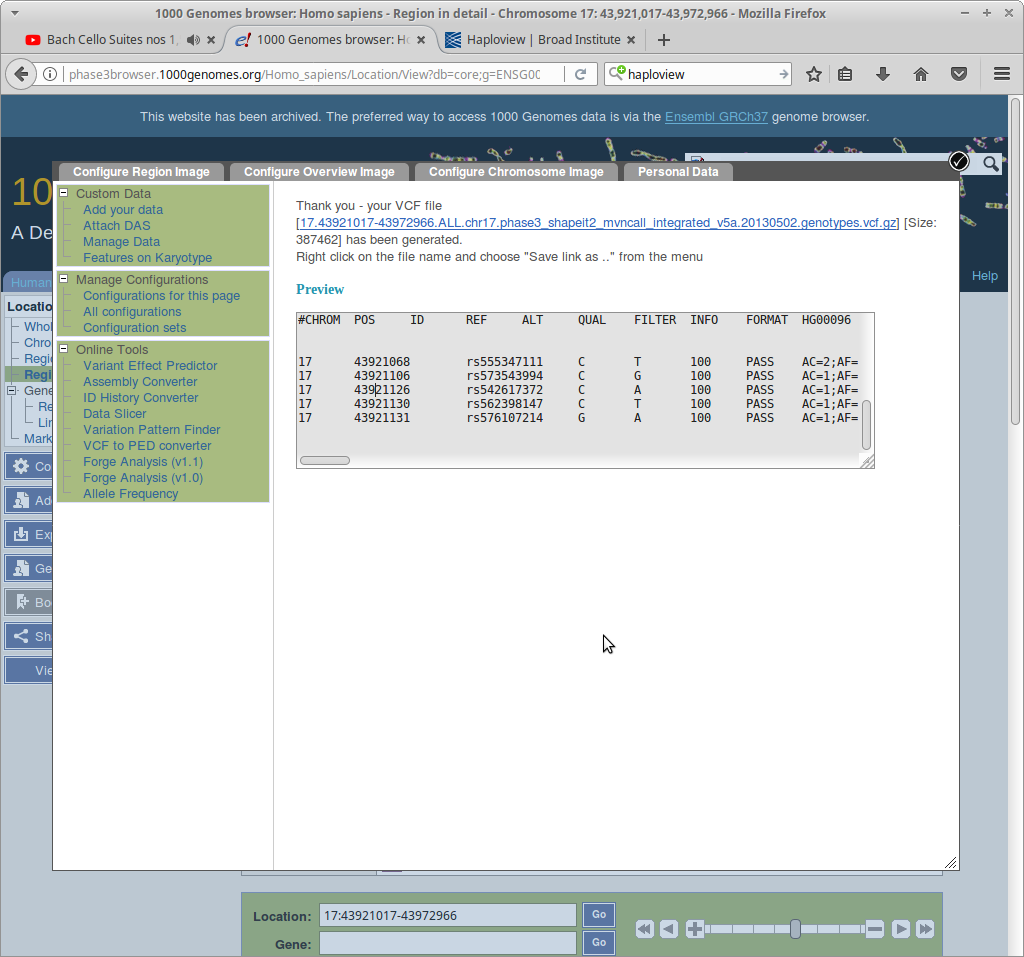
\includegraphics[width=.7\linewidth]{vcf1.png}
\end{center}
\end{figure}

\end{frame}



\begin{frame}[fragile]
\frametitle{1000 Genomes}
Formato VCF
\begin{figure}[htbp]
\begin{center}
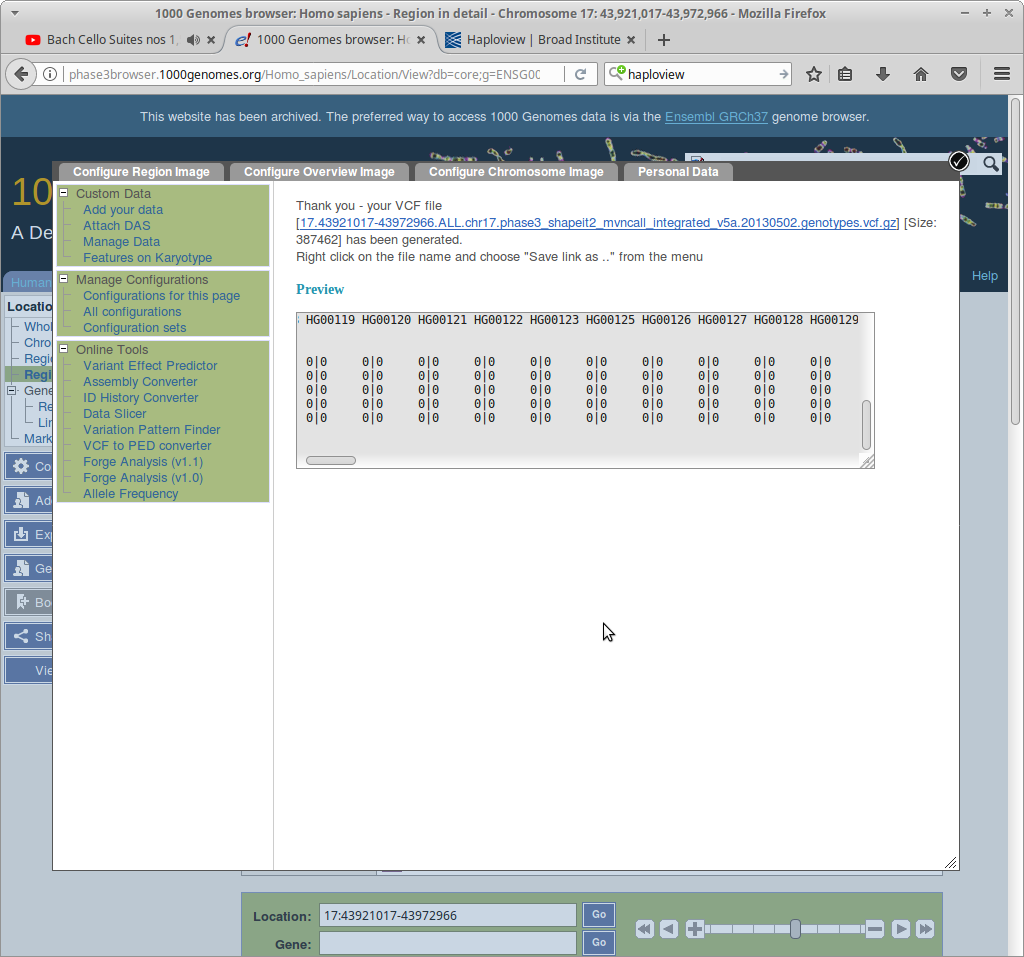
\includegraphics[width=.7\linewidth]{vcf2.png}
\end{center}
\end{figure}
\end{frame}



\begin{frame}[fragile]
\frametitle{Bioconductor}
Paquete Variant Annotation para leer datos VCF
\begin{figure}[htbp]
\begin{center}
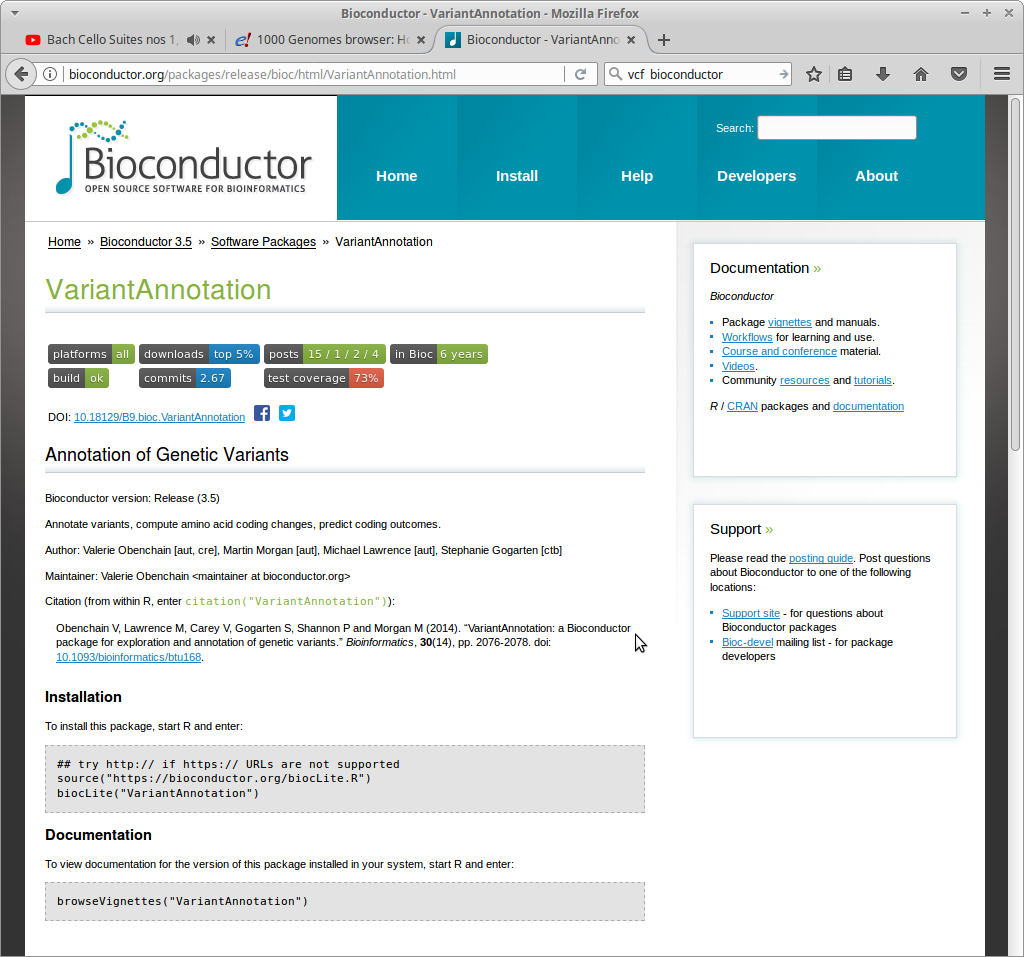
\includegraphics[width=.7\linewidth]{variantaanot.png}
\end{center}
\end{figure}
\end{frame}


\begin{frame}[fragile]
\frametitle{VCF in R}

se pueden cargar los binarios snp.RData
\begin{knitrout}\footnotesize
\definecolor{shadecolor}{rgb}{0.969, 0.969, 0.969}\color{fgcolor}\begin{kframe}
\begin{alltt}
\hlkwd{source}\hlstd{(}\hlstr{"http://bioconductor.org/biocLite.R"}\hlstd{)}
\hlkwd{biocLite}\hlstd{(}\hlstr{"VariantAnnotation"}\hlstd{)}
\end{alltt}
\end{kframe}
\end{knitrout}
\end{frame}



\begin{frame}[fragile]
\frametitle{Bioconductor}
Variant annotation
\begin{figure}[htbp]
\begin{center}
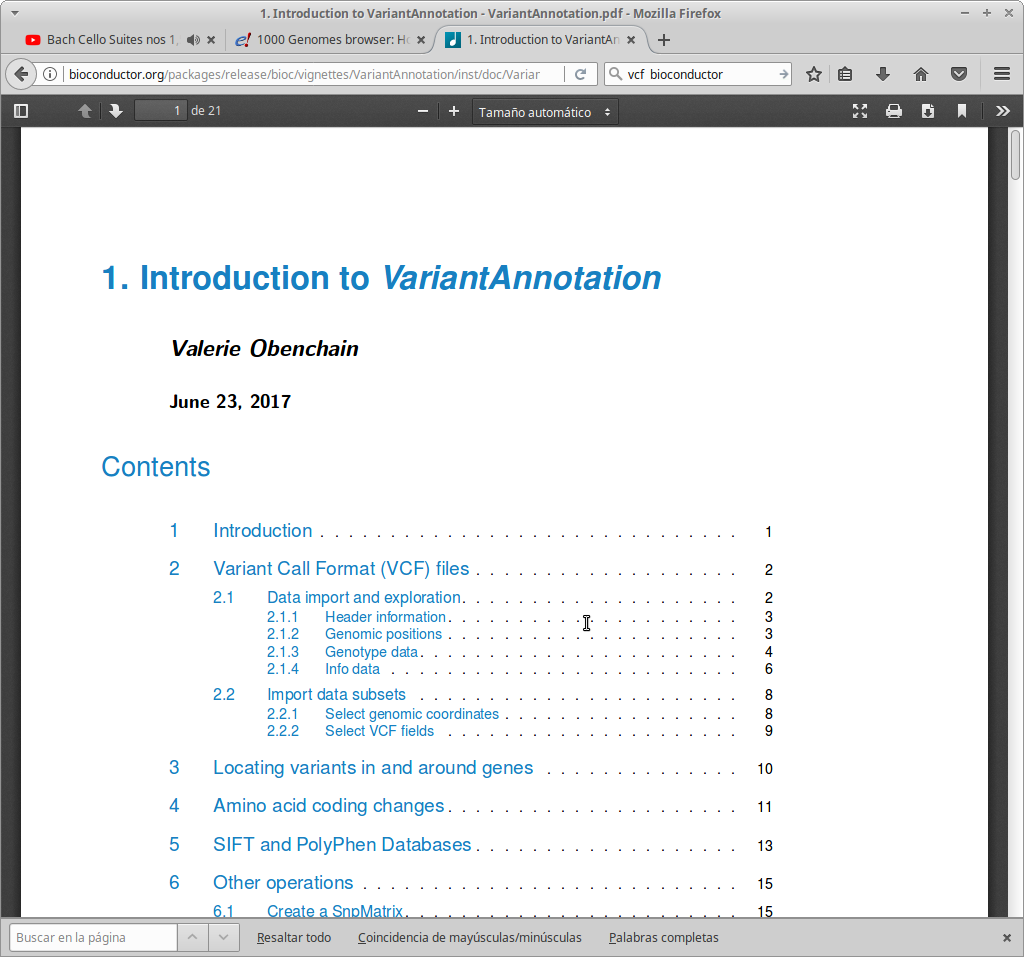
\includegraphics[width=.7\linewidth]{vineta.png}
\end{center}
\end{figure}
\end{frame}


\begin{frame}[fragile]
\frametitle{VCF in R}

\begin{knitrout}\footnotesize
\definecolor{shadecolor}{rgb}{0.969, 0.969, 0.969}\color{fgcolor}\begin{kframe}
\begin{alltt}
\hlkwd{library}\hlstd{(VariantAnnotation)}
\hlstd{fl}\hlkwb{<-}\hlstr{"datos/17.43921017-43972966.ALL.chr17.phase3_shapeit2_mvncall_integrated_v5a.20130502.genotypes.vcf"}
\hlstd{vcf} \hlkwb{<-} \hlkwd{readVcf}\hlstd{(fl,} \hlstr{"hg19"}\hlstd{)}
\hlstd{vcf}
\end{alltt}
\begin{verbatim}
## class: CollapsedVCF 
## dim: 1863 2504 
## rowRanges(vcf):
##   GRanges with 5 metadata columns: paramRangeID, REF, ALT, QUAL, FILTER
## info(vcf):
##   DataFrame with 27 columns: CIEND, CIPOS, CS, END, IMPRECISE, MC, MEIN...
## info(header(vcf)):
##                  Number Type    Description                               
##    CIEND         2      Integer Confidence interval around END for impr...
##    CIPOS         2      Integer Confidence interval around POS for impr...
##    CS            1      String  Source call set.                          
##    END           1      Integer End coordinate of this variant            
##    IMPRECISE     0      Flag    Imprecise structural variation            
##    MC            .      String  Merged calls.                             
##    MEINFO        4      String  Mobile element info of the form NAME,ST...
##    MEND          1      Integer Mitochondrial end coordinate of inserte...
##    MLEN          1      Integer Estimated length of mitochondrial insert  
##    MSTART        1      Integer Mitochondrial start coordinate of inser...
##    SVLEN         .      Integer SV length. It is only calculated for st...
##    SVTYPE        1      String  Type of structural variant                
##    TSD           1      String  Precise Target Site Duplication for bas...
##    AC            A      Integer Total number of alternate alleles in ca...
##    AF            A      Float   Estimated allele frequency in the range...
##    NS            1      Integer Number of samples with data               
##    AN            1      Integer Total number of alleles in called genot...
##    EAS_AF        A      Float   Allele frequency in the EAS populations...
##    EUR_AF        A      Float   Allele frequency in the EUR populations...
##    AFR_AF        A      Float   Allele frequency in the AFR populations...
##    AMR_AF        A      Float   Allele frequency in the AMR populations...
##    SAS_AF        A      Float   Allele frequency in the SAS populations...
##    DP            1      Integer Total read depth; only low coverage dat...
##    AA            1      String  Ancestral Allele. Format: AA|REF|ALT|In...
##    VT            .      String  indicates what type of variant the line...
##    EX_TARGET     0      Flag    indicates whether a variant is within t...
##    MULTI_ALLELIC 0      Flag    indicates whether a site is multi-allelic 
## geno(vcf):
##   SimpleList of length 1: GT
## geno(header(vcf)):
##       Number Type   Description
##    GT 1      String Genotype
\end{verbatim}
\end{kframe}
\end{knitrout}
\end{frame}

\begin{frame}[fragile]
\frametitle{VCF in R}
\begin{knitrout}\footnotesize
\definecolor{shadecolor}{rgb}{0.969, 0.969, 0.969}\color{fgcolor}\begin{kframe}
\begin{alltt}
\hlstd{genos}\hlkwb{<-}\hlkwd{geno}\hlstd{(vcf)}
\hlkwd{names}\hlstd{(genos)}
\end{alltt}
\begin{verbatim}
## [1] "GT"
\end{verbatim}
\begin{alltt}
\hlkwd{dim}\hlstd{(genos}\hlopt{$}\hlstd{GT)}
\end{alltt}
\begin{verbatim}
## [1] 1863 2504
\end{verbatim}
\begin{alltt}
\hlstd{genos}\hlopt{$}\hlstd{GT[}\hlnum{1}\hlopt{:}\hlnum{5}\hlstd{,}\hlnum{1}\hlopt{:}\hlnum{5}\hlstd{]}
\end{alltt}
\begin{verbatim}
##             HG00096 HG00097 HG00099 HG00100 HG00101
## rs555347111 "0|0"   "0|0"   "0|0"   "0|0"   "0|0"  
## rs573543994 "0|0"   "0|0"   "0|0"   "0|0"   "0|0"  
## rs542617372 "0|0"   "0|0"   "0|0"   "0|0"   "0|0"  
## rs562398147 "0|0"   "0|0"   "0|0"   "0|0"   "0|0"  
## rs576107214 "0|0"   "0|0"   "0|0"   "0|0"   "0|0"
\end{verbatim}
\end{kframe}
\end{knitrout}

Si el archivo es grande readVcf permite leer s\'olo regiones de interes
\end{frame}



\begin{frame}[fragile]
\frametitle{VCF in R}

Los genotipos en formato 0,1,2 pueden ser encontrados en $genos\$DS$.

Si no se puede entonces se puede calcular asi

\begin{knitrout}\footnotesize
\definecolor{shadecolor}{rgb}{0.969, 0.969, 0.969}\color{fgcolor}\begin{kframe}
\begin{alltt}
\hlstd{snps}\hlkwb{<-}\hlstd{genos}\hlopt{$}\hlstd{GT}
\hlstd{snps[snps}\hlopt{==}\hlstr{"0|0"}\hlstd{]}\hlkwb{<-}\hlnum{0}
\hlstd{snps[snps}\hlopt{==}\hlstr{"1|1"}\hlstd{]}\hlkwb{<-}\hlnum{2}
\hlstd{snps[snps}\hlopt{!=}\hlnum{0} \hlopt{&} \hlstd{snps} \hlopt{!=}\hlnum{2}\hlstd{]}\hlkwb{<-}\hlnum{1}
\hlstd{snps[}\hlnum{1}\hlopt{:}\hlnum{5}\hlstd{,}\hlnum{1}\hlopt{:}\hlnum{5}\hlstd{]}
\end{alltt}
\begin{verbatim}
##             HG00096 HG00097 HG00099 HG00100 HG00101
## rs555347111 "0"     "0"     "0"     "0"     "0"    
## rs573543994 "0"     "0"     "0"     "0"     "0"    
## rs542617372 "0"     "0"     "0"     "0"     "0"    
## rs562398147 "0"     "0"     "0"     "0"     "0"    
## rs576107214 "0"     "0"     "0"     "0"     "0"
\end{verbatim}
\begin{alltt}
\hlkwd{save}\hlstd{(snps,} \hlkwc{file}\hlstd{=}\hlstr{"snpsMAPT.RData"}\hlstd{)}
\end{alltt}
\end{kframe}
\end{knitrout}


\end{frame}


\begin{frame}[fragile]
\frametitle{VCF in snpStats}
snpStats usa formato 1,2,3 para genotipos y el 0 para missing
\begin{knitrout}\footnotesize
\definecolor{shadecolor}{rgb}{0.969, 0.969, 0.969}\color{fgcolor}\begin{kframe}
\begin{alltt}
\hlkwd{library}\hlstd{(snpStats)}
\hlstd{snpsnew}\hlkwb{<-}\hlkwd{t}\hlstd{(snps)}
\hlstd{snpsnew[snps}\hlopt{==}\hlstr{"0"}\hlstd{]} \hlkwb{<-} \hlnum{1}
\hlstd{snpsnew[snps}\hlopt{==}\hlstr{"1"}\hlstd{]} \hlkwb{<-} \hlnum{2}
\hlstd{snpsnew[snps}\hlopt{==}\hlstr{"2"}\hlstd{]} \hlkwb{<-} \hlnum{3}

\hlstd{snpsSNPstats} \hlkwb{<-} \hlkwd{new}\hlstd{(}\hlstr{"SnpMatrix"}\hlstd{, snpsnew)}
\end{alltt}
\begin{verbatim}
## coercing object of mode  character  to SnpMatrix
\end{verbatim}
\begin{alltt}
\hlkwd{print}\hlstd{(}\hlkwd{as}\hlstd{(snpsSNPstats[}\hlnum{1}\hlopt{:}\hlnum{5}\hlstd{,}\hlnum{1}\hlopt{:}\hlnum{5}\hlstd{],} \hlstr{'character'}\hlstd{))}
\end{alltt}
\begin{verbatim}
##         rs555347111 rs573543994 rs542617372 rs562398147 rs576107214
## HG00096 "A/A"       "A/A"       "A/A"       "A/A"       "A/A"      
## HG00097 "A/A"       "A/A"       "A/A"       "A/A"       "A/A"      
## HG00099 "A/A"       "A/A"       "A/A"       "A/A"       "A/A"      
## HG00100 "A/A"       "A/A"       "A/A"       "A/A"       "A/A"      
## HG00101 "A/A"       "A/A"       "A/A"       "A/A"       "A/A"
\end{verbatim}
\begin{alltt}
\hlkwd{save}\hlstd{(snpsSNPstats,} \hlkwc{file}\hlstd{=}\hlstr{"snpsSNPstats.RData"}\hlstd{)}
\end{alltt}
\end{kframe}
\end{knitrout}

\end{frame}



\begin{frame}[fragile]
\frametitle{1000 Genomes}
Los datos de los 1000 genomas (y HapMap)tambien est\'an en formato PLINK por chromosomas
\begin{figure}[htbp]
\begin{center}
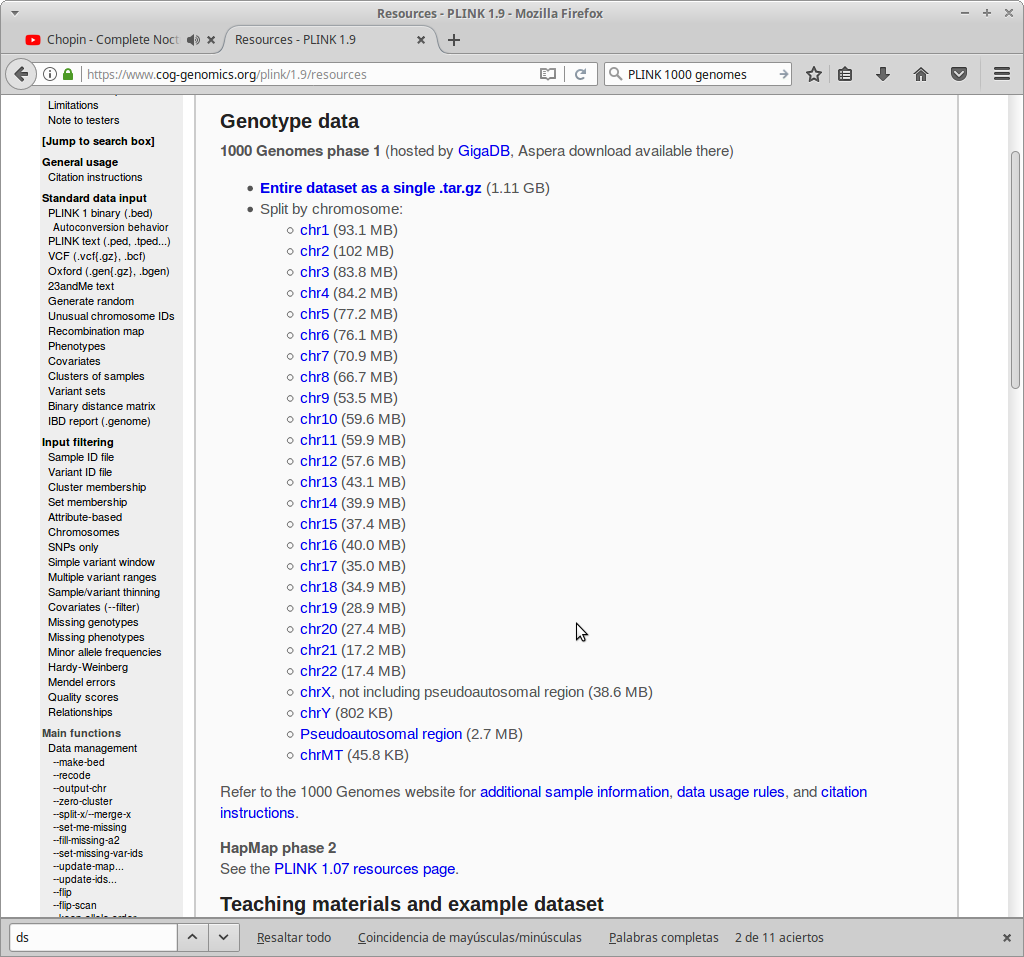
\includegraphics[width=.7\linewidth]{plink1kgenomes.png}
\end{center}
\end{figure}

\end{frame}


\begin{frame}[fragile]
\frametitle{PLINK a VCF}
\begin{itemize}
\item los comandos PLINK puden usar formato VCF
\item tambi\'en se puede convertir .bed .bim .fam a formato a VCF y vise-versa
\end{itemize}

{\scriptsize
\begin{verbatim}
$ plink --bfile [filename prefix] --recode vcf --out [VCF prefix]
$ plink --vcf [VCF filename] --out [.bed/.bim/.fam prefix]
\end{verbatim}
}

\end{frame}

\begin{frame}[fragile]
\frametitle{Ejercicio}
\begin{itemize}
\item Descargar datos de los 1000 Genomas en PLINK 
\item leerlos en snpStats
\item si PLINK est\'a instalado convertirlos en VCF
\item leerlos en snpStats
\end{itemize}
\end{frame}

\end{document}
